\section{Motivation}

More and more people consume media from client-server based sources (e.g., Facebook, Netflix, Spotify, etc.) instead of traditional one-to-many sources (e.g., television, radio, etc.) that usually carry emergency alerts. The current solution to alerting users of client-server systems is to provide an emergency alert feed that websites and providers can periodically poll and then push to users. While television and radio broadcasters (and providers) are legally required to disseminate these messages, websites and ISPs\footnote{Companies that provide both (like AT\&T), only are required to send via the mandated medium} are not.\cite{cfr47}

More importantly, the existing systems treat the internet as a reliable black box, ignoring the increasing frequency and strength of cyber-attacks. In 'traditional' emergency scenarios the internet is either present or not; physical cables are down or up. But in a denial of service attack, the physical infrastructure is intact, and the ability for useful communication is heavily degraded. In a scenario where either terrorist or state actors decide to attack in both the physical \textit{and} cyber realms, citizens still need to be able to receive these critical alerts.

\section{Background}
\subsection{Trotsky}
The foundation for this project is Trotsky, a clean-slate internet framework that separates intra (L3) and inter (L3.5) domain abstractions, and allows for a proliferation of specialized network architectures. The forwarding appliance in Trotsky is the Trotsky Processor (TP): an end-point for an L3.5 pipe that forwards based on the L3.5 protocol agent of the incoming packet. New inter-domain architectures can be developed and deployed by simply adding a routing agent to TPs. In addition, new intra-domain architectures can be created and replaced within a domain without affecting the L3.5 architecture.

We leverage Trotsky both as a way of deployment and as a rationale for our design. Deployment in Trotsky is as simple as pushing a software update to TPs. We also use the L3.5 abstraction of domain-to-domain communication to simplify the problem from sending a message to every end-host to sending a message to every ISP. We aim to solve one specific problem: \textit{emergency} broadcast---with Trotsky this is allowed and even encouraged. There is no reason to add complexity to existing architectures or create a new all-encompassing architecture because Trotsky allows for an ecosystem of specialized architectures. 

\subsection{Existing Infrastructure}\label{infrabckgrnd}
The US public alert system has been around for over half a century\footnote{This paper focuses on the US, but most countries (if they have such systems) have similar designs.}. The system begins with FEMA initiating an alert and sending it to Primary Entry Points (PEPs) across the country via robust RF communication. PEPs are hardened sites that help spread the alert to local radio and TV stations (and can also serve is origin points for local alerts). FEMA (at the same time as the aforementioned broadcast) publishes alerts to an online information feed. All cellular providers and, as seen in a 2018 test of the system, a majority of radio \& television providers use this online feed. Ultimately, the FEMA message first goes to distributors, which then, in turn, deliver the alert to individual citizens. \cite{ipaws101}

The 2018 system test showed some interesting results about the effectiveness of the system. Overall only about 80\% of people received the alert, showing that there is room for improvement. Furthermore, most people that were surveyed received the alert on their smartphone, rather than radio or television (combined less than 10\% of respondents ). The cellular transmission caused a variety of issues, ranging from ensuring service outages, to receipt of dozens of duplicate alerts.\cite{weatest,everbridge}

\section{Design Overview}
Our design combines the abstractions provided by Trotsky with the hierarchical broadcast design provided by the current emergency broadcast infrastructure. Concretely, this means flooding an alert on L3.5, and then having ISPs push the message to citizens. 

\begin{figure}[tp]
\centering
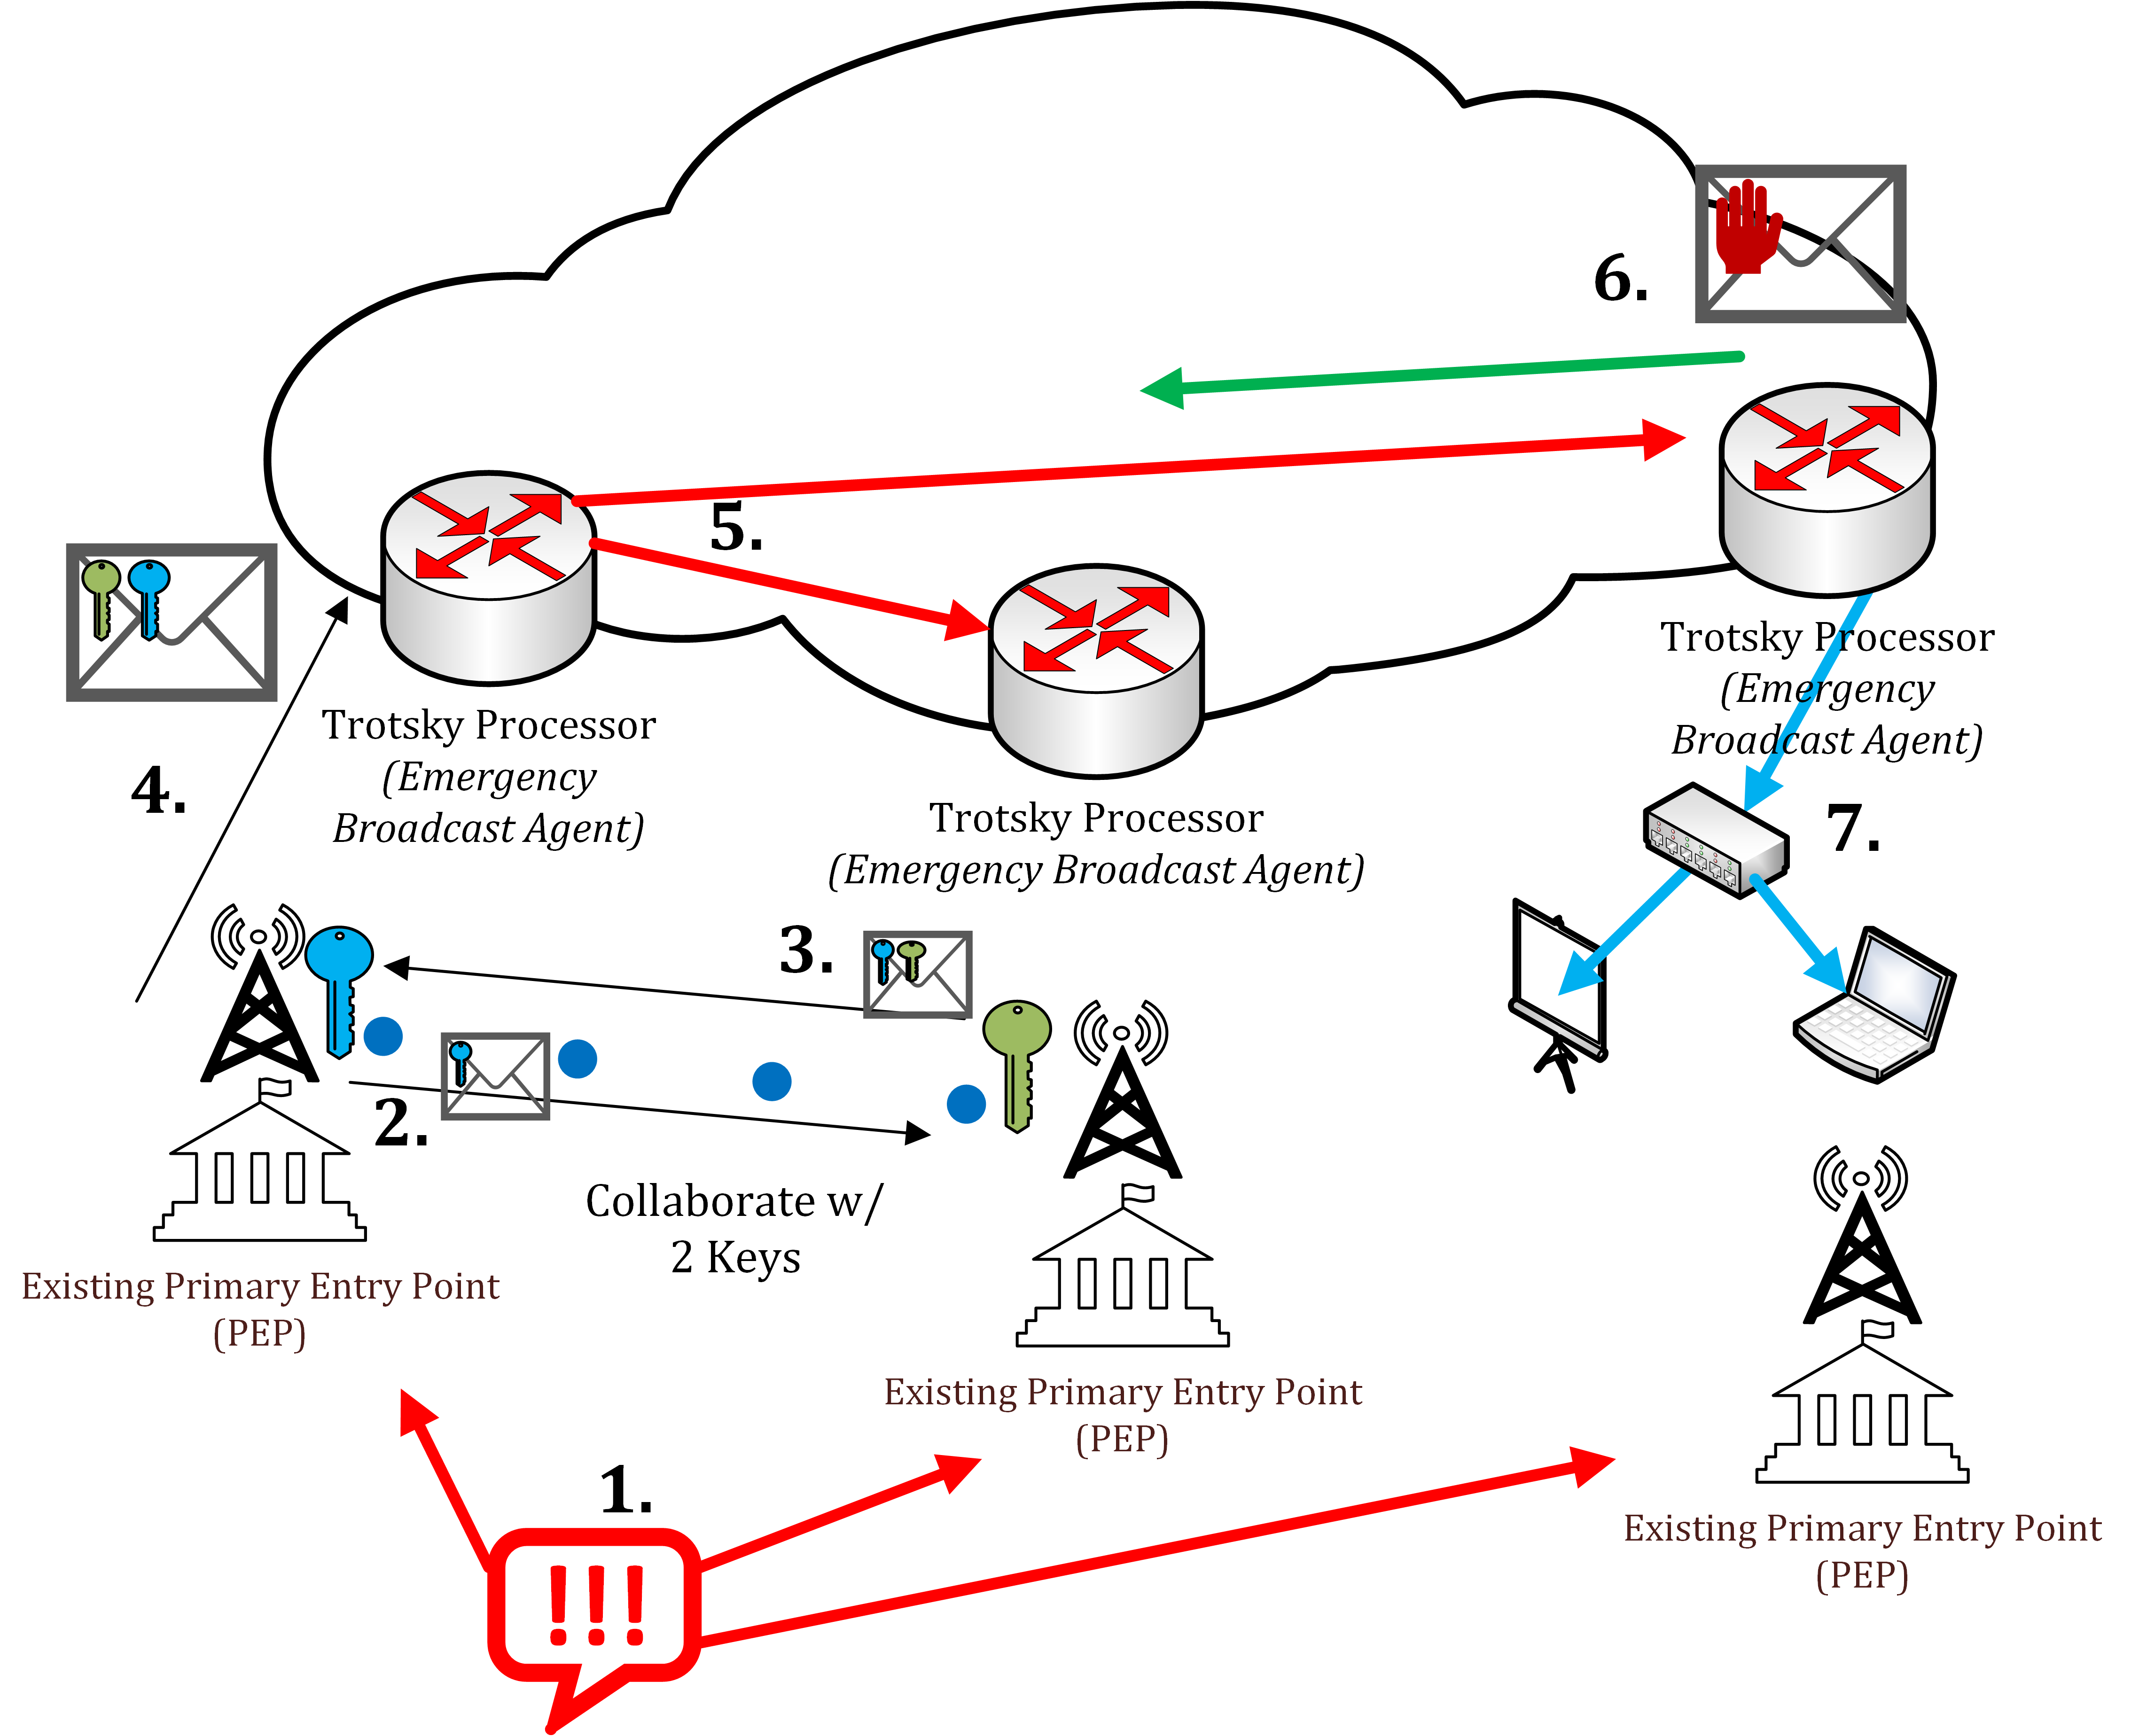
\includegraphics[width=8.5cm]{figures/full_diagram_v2.png}
\caption{Step-by-step process of a nation-wide broadcast}
\label{fig:brdcast}
\end{figure}


\subsection{Detailed Proposed Process}
The steps for a national alert solution using our proposed architecture are shown in Figure \ref{fig:brdcast}, and are described in detail below.

\textbf{1.} Some approved entity sends an out-of-band signed message to the PEPs\footnote{These are the same PEPs mentioned in section \ref{infrabckgrnd}} across the country. This step helps ensure that the message is inserted into multiple points of the internet, reducing the impact of network partition. 

\textbf{2. \& 3.} PEPs confer with each other (out-of-band) to reduce the risk of a compromised PEP (described in section \ref{acl}). 

\textbf{4.} PEPs then send the message to their ISP where the first TP receives the message. The TP ensures that the message has the correct signature (described in section \ref{acl}), dropping the message if it does not.

\textbf{5.} The TP initiates L3.5 flooding\footnote{Continual broadcast to all neighbors.} of the packetized message, encoding the data using a fountain code (described in section \ref{reliable}). Every TP that receives a packet from the message \textit{also checks} the signature before forwarding. If the signature does not match, the packet is dropped.

\textbf{6.} Each TP floods until its neighbor responds with 'Message Received.' 

\textbf{7.} When each TP is able to decode the message, the owner of the TP (an ISP) will begin internal, intra-domain broadcast to its customers.

\\
Once messages get to an ISP, the ISP is responsible for the 'last-mile' delivery to people. This delivery service can differ domain to domain. For a wireless provider, they may use the same SMS-based emergency alert system that is in use today. ISPs can use multicast, existing modem communication systems, or whatever technologies they may have. Finally, the host-based delivery is as simple as having browsers or OS vendors accepting special, verified 'alert' packets. 

A local emergency broadcast would follow a similar procedure, but still differs in two main ways. First, it may not require cross validation with other PEPs. This is because a locality may only have one PEP, and an initiating authority would go directly to that PEP for broadcasting. Second, when the message is flooded on L3.5, TPs in different localities would not continue the broadcast\footnote{If a TP knew its neighbors were in the same location as the broadcast, it would forward the packets.}. 

To draw our discussion of the overall design to a close, we will now discuss how the packet layout enables the functionality of our architecture. The fields in the packet are shown in Figure \ref{fig:pckt}; everything 'inside' of the L3.5 header was created as part of our proposal. The L3.5 header specifies that the TP should pass the packet to the Emergency Broadcast processing agent. The\textit{ Broadcast ID} is a  flow number to differentiate between messages. The \textit{Total Number Sent} specifies how many packets the TP should receive before sending 'Message Received.' This will be larger than the number of needed for decoding the message and will be described in section \ref{reliable}. \textit{Location} specifies what region\footnote{Any standardized location format works (e.g., ZIP code, city, etc.)} the message is for, enabling local broadcast. The \textit{Time Stamp} and \textit{Crypto Signature} are used in verification and in preventing replay-based attacks (messages with a valid signature and a stale time stamp will be dropped).
\begin{figure}[tp]
\centering
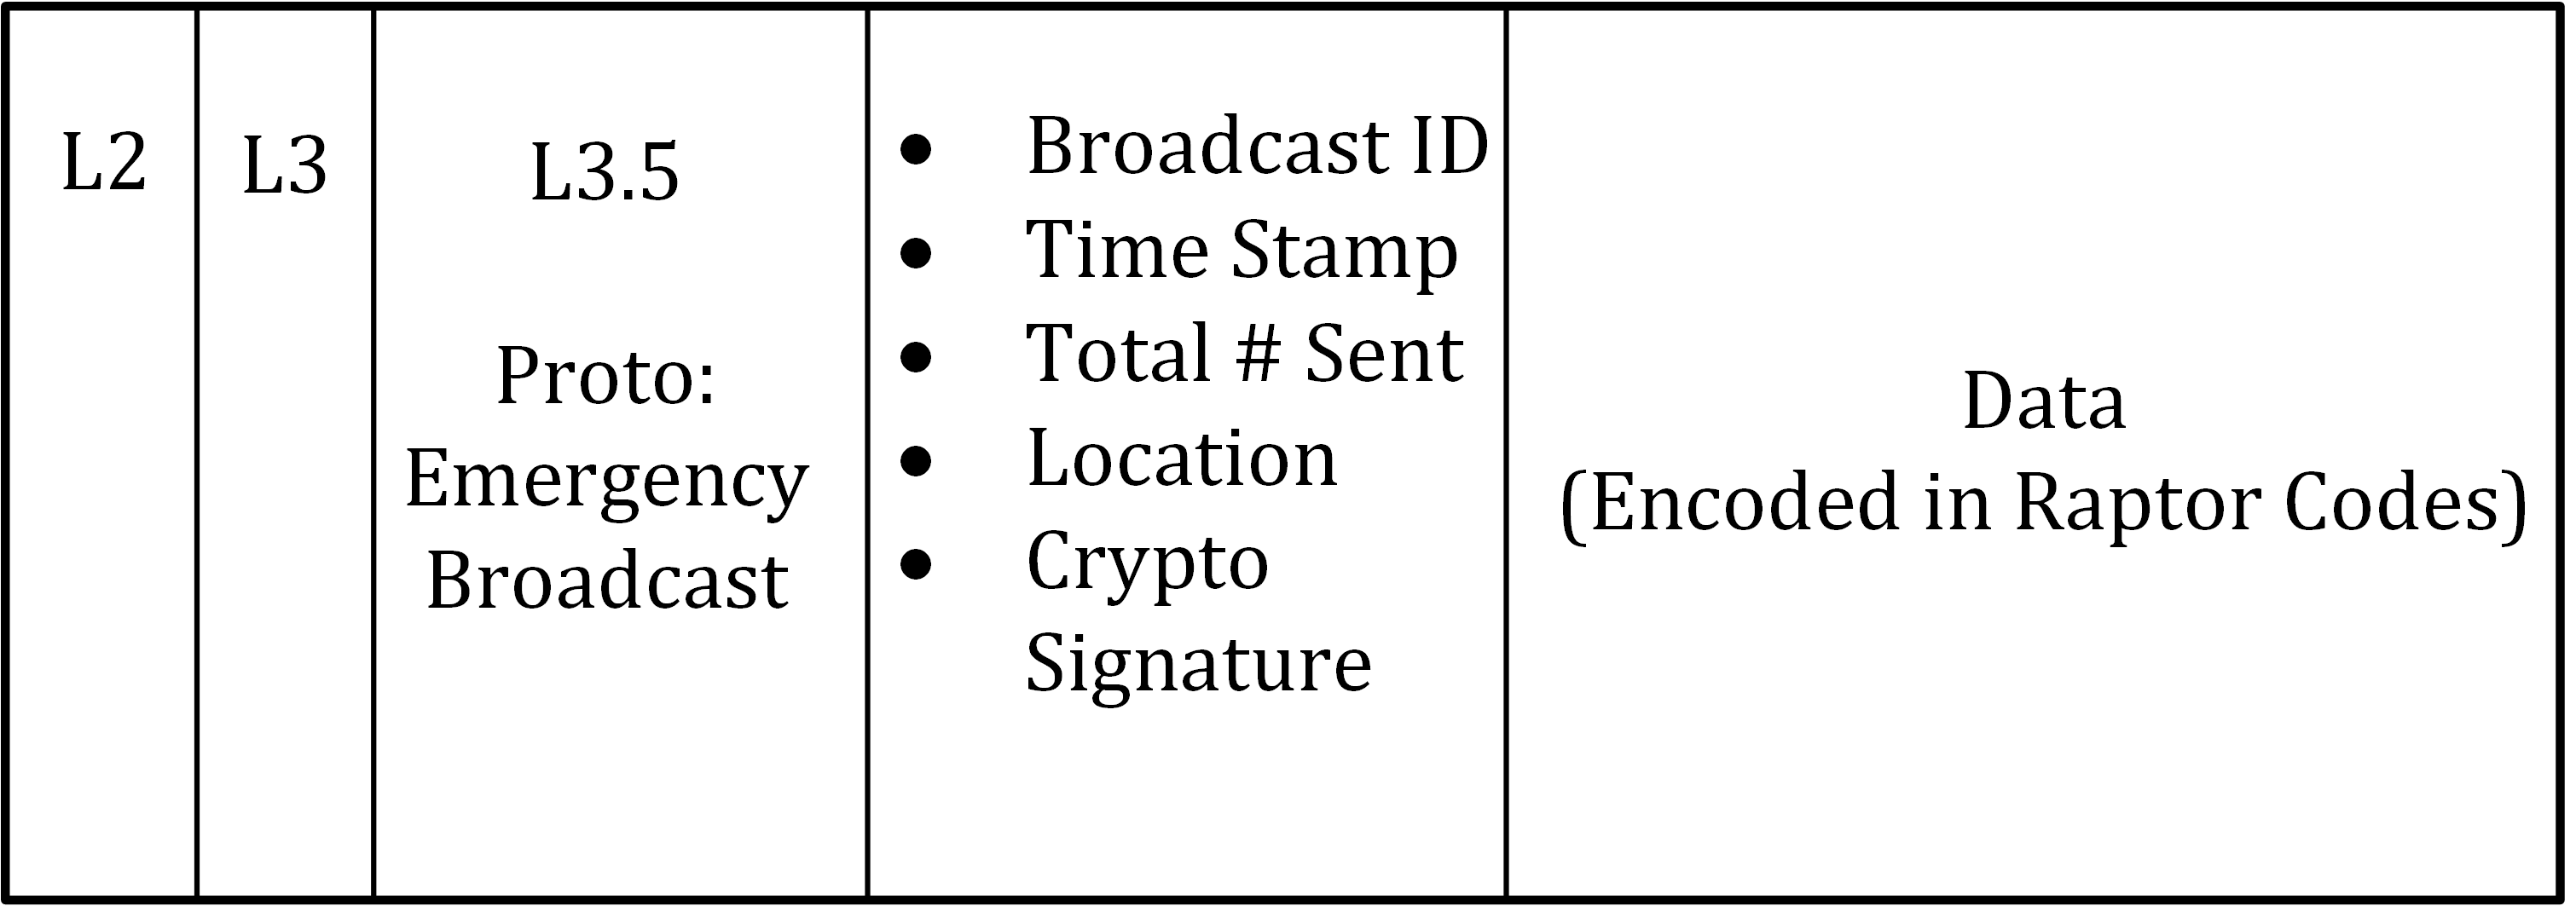
\includegraphics[width=8.5cm]{figures/packet_header.png}
\caption{Packet layout}
\label{fig:pckt}
\end{figure}

\subsection{Rationale}
The goal for this architecture is two-fold: \textbf{1)} robust message delivery and \textbf{2)} access control. We further worked with several key assumptions:  \textbf{A)} emergency broadcasts are relatively infrequent, \textbf{B)} Trotsky is the standard framework, and \textbf{C)} some central authority that must be trusted\footnote{This is meant in both having some sort of centralized key storage and also in the sense of having someone with absolute ability to launch an alert (the president)}. This prioritization led to the design we have here.  

Goal \textbf{1} and assumptions \textbf{B} allowed us to consider in-networks solutions. End-to-end arguments over many lossy links\footnote{While the internet is usually \textit{not} lossy, in congestion-attack scenarios that we are concerned with, packet loss is common.} are weak because the per-link drop-probabilities are compounded and result in low chance of delivery. Trotsky allows us to place functionality in the network, reducing the number of links between logical endpoints, increasing robustness. In network support also allows for extensions like increasing QoS levels for these alerts\footnote{To reiterate: this is an extension.}. 

Goal \textbf{1} and assumption \textbf{A} led us to the idea of flooding. This architecture is used for infrequent and \textit{urgent} events, meaning that degradation of other traffic is tolerable. Using BGP (or any 'normal' inter-domain routing) paths increase the probability of message failure if links go down or are unstable; it also introduces unnecessary complexity. The use of many PEPs to introduce the message to the system also reduces the single-point-of-failure of having a truly centralized network entry point.

In the following section, we will focus on goal \textbf{2} and assumption \textbf{C}. 
\section{Access Control}\label{acl}
\subsection{Overview}

\subsection{Threat Model}
\subsection{Extensions}
\section{Reliable Transmission}\label{reliable}
In order to increase the speed and reliability of message transmission, we will use RaptorQ fountain codes. The idea of fountain codes is that a finite source of $k$ symbols can be transformed into an arbitrarily long stream of non-redundant symbols. Furthermore, the receiver only needs to receive \textbf{any} $k + \epsilon$ symbols to recover the original message. For RaptorQ, $\epsilon = 0$ and $\epsilon = 2$ give, respectively, a $99\%$ and $99.9999\%$ chance of recovery.\cite{raptorq, raptorqpresent}

RaptorQ encoding also provides high performance through linear time encoding and decoding, reducing the burden on TPs\footnote{Specifically that the encoding/decoding scheme does not rely on specialized hardware}. Codornices, a RaptorQ package from ICSI, recently released performance results. For a 128 kB message on x86, the encode and decode took under $0.5$ ms each, and was able to produce/consume at a rate of $2$ Gbps\cite{raptorqperf}. This performance is definitely sufficient for our application, as will be described in the following section.
\subsection{Use in our system}
-   Send  $2\cdot k_{overshoot}$

-   Encode once (at transmission)

-   Downside of no-blocking

- Consideration of ACK-based as well


\section{Evaluation}
For our evaluation we used the python networkx library to model the high level behavior of different propagation modes.\cite{nwx}
For network topologies, we used an abridged Rocketfuel ISP level map. \cite{rocketfuel}

\begin{figure}[tp]
\centering
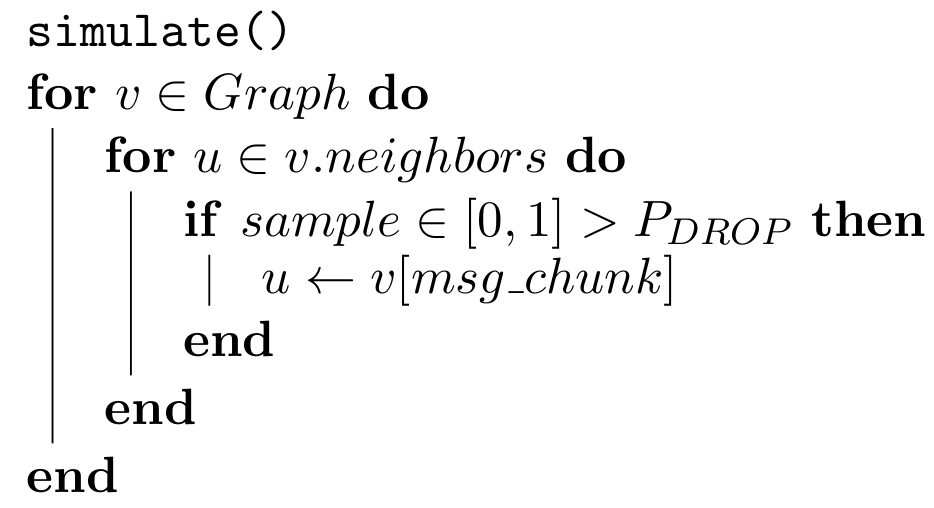
\includegraphics[width=6cm]{figures/simulate_algo.png}
\caption{Basic simulation algorithm used}
\label{algo:a1}
\end{figure}

\subsection{Simulation Design}
The test framework is described in Figure \ref{algo:a1}. Special care is taken to ensure that if a node gets a chunk on one iteration, it cannot transmit until the next iteration. The simulation continues until every node has received all packets in the message.  

To model the RaptorQ encoding technique, each node iterates through all received packets and sends one (not knowing what the reciever has). The first node is given more chunks than the message needs to simulate the infinite generation of blocks. In the case of the blocking version, each node waits until it had received enough chunks (the number of chunks in the message) to decode a message before sending. For the ACK-based sending technique, each node keeps track of the largest 'sequence number' that each neighbor has received. It repeatedly sends one chunk until the neighbor tells it to move to the next block.

\subsection{Experimental Setup}
For each experiment we defined a link-based drop probability value, selected a given propagation method and ran the simulation. For each set of control variables we repeated the simulation 100 times to get a stronger sample size. For all experiments, we selected one sender node (at random from the graph) and sent a 15-packet-long message.

We were only concerned with relative performance of methods, not absolute performance. Drops were used to model congestion because routing devices under attack would begin dropping packets once buffers filled up. Latency was ignored because the only component of latency that would change between methods is the number of packets sent (propagation, queuing delays would be the same).

\subsection{Results}

\begin{figure}[tp]
\centering
\noindent
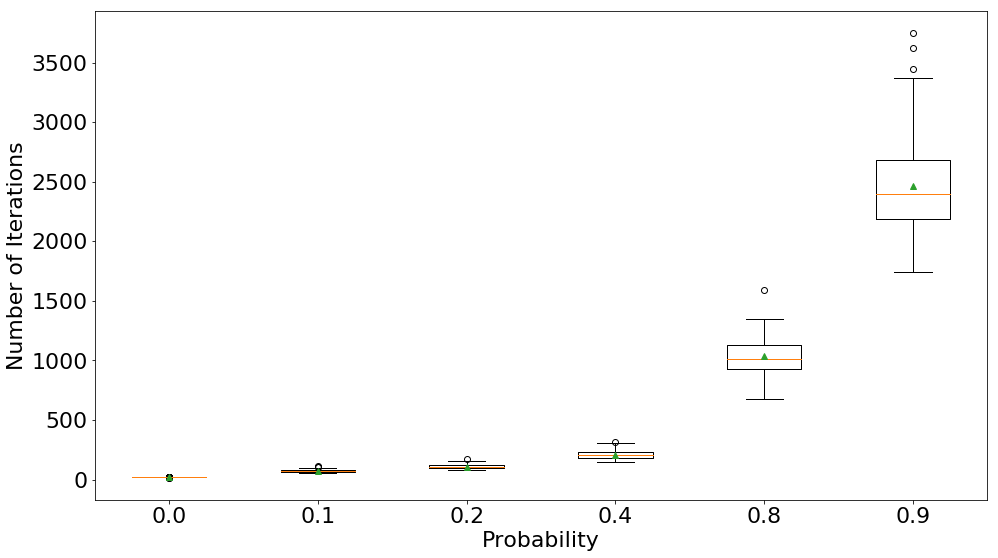
\includegraphics[width=8cm]{figures/big_font/ack_trim.png}
\caption{Box-and-Whisker plot of the ACKing sender }
\label{graph:ack}
\end{figure}

\begin{figure}[tp]
\centering
\noindent
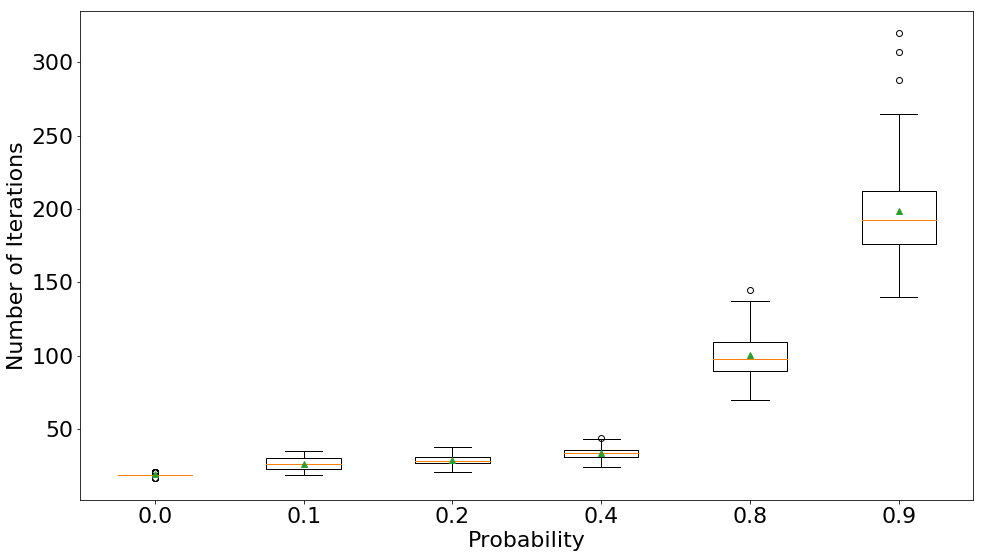
\includegraphics[width=8cm]{figures/big_font/rateless_trim.png}
\caption{Box-and-Whisker plot of the Rateless sender}
\label{graph:rateless}
\end{figure}


Our results are summarized in Figures \ref{graph:ack}, \ref{graph:rateless},\ref{graph:ackvsrateless}, \ref{graph:blockingvsnot}, and \ref{graph:ackvsratelessLOG} \footnote{Note that the drop probability of $0.99$ was excluded from Figure \ref{graph:ack} and Figure \ref{graph:rateless} in order to increase readability.}.

The first two show the performance of the ACK-based sender and rateless sender relative to themselves as the probability of packet-loss increases. From these graphs, we can see how the message propagation time would vary based on the severity of packet loss. These graphs provide a stand-alone baseline for each sending method.  

The first two show the variance of performance of the ACK-based sender and the rateless sender as probability of packet loss increases. The latter three directly compare the performance of the rateless (non-blocking) sender with the performance of the ACK-based sender and rateless, blocking sender. 

The rateless outperforms the ACKing one in almost all scenarios. In Figure \ref{graph:ackvsrateless}, the huge increase in loss for ACK-Based is quite apparent. It performs substantially worse when conditions become severely degraded. Figure \ref{graph:ackvsratelessLOG} shows that even for more mild conditions, the rateless sender is almost 10x better.

We were initially unsure about whether we should immediately send packets to neighbors or wait for an entire message to begin sending. Figure \ref{graph:blockingvsnot} shows that the version that immediately sends always outperforms the blocking version. The improvement is always present, but becomes especially present when probability of loss increases. It should be noted that the both rateless senders are far better than the ACKing sender.

Overall the results are not surprising. The rateless sender benefits from being able to send for the longest amount of time (even if it is only repeatedly sending one block). The ACK-based sender takes a double hit from lossy links, and thus has a severe performance degradation. The blocking, rateless sender suffers from having to wait longer to begin transmitting; this surprisingly is not that much for all but the most extreme drop rates.

\begin{figure}[tp]
\centering
\noindent
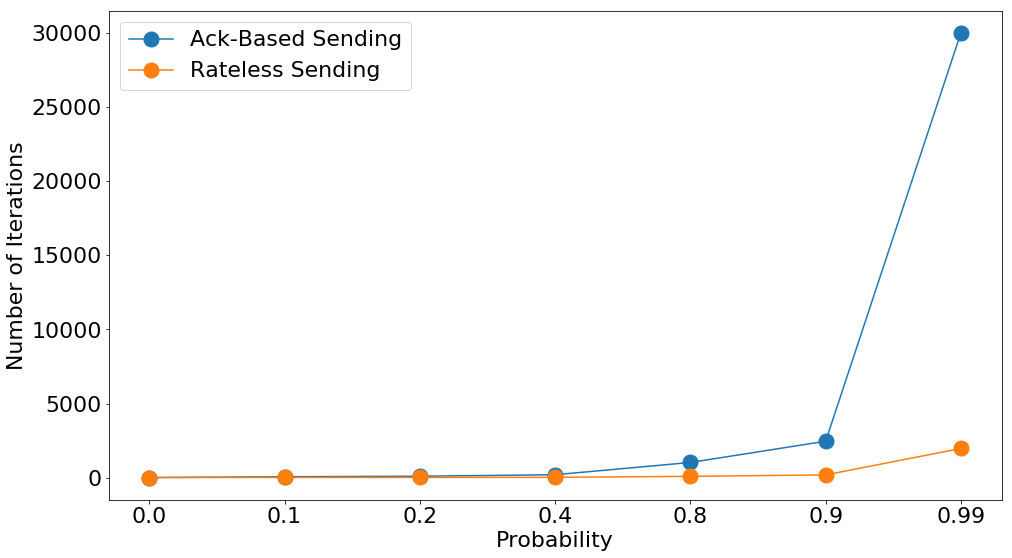
\includegraphics[width=8cm]{figures/big_font/ack_comp.png}
\caption{Comparison of the ACKing and Rateless senders}
\label{graph:ackvsrateless}
\end{figure}


\begin{figure}[tp]
\centering
\noindent
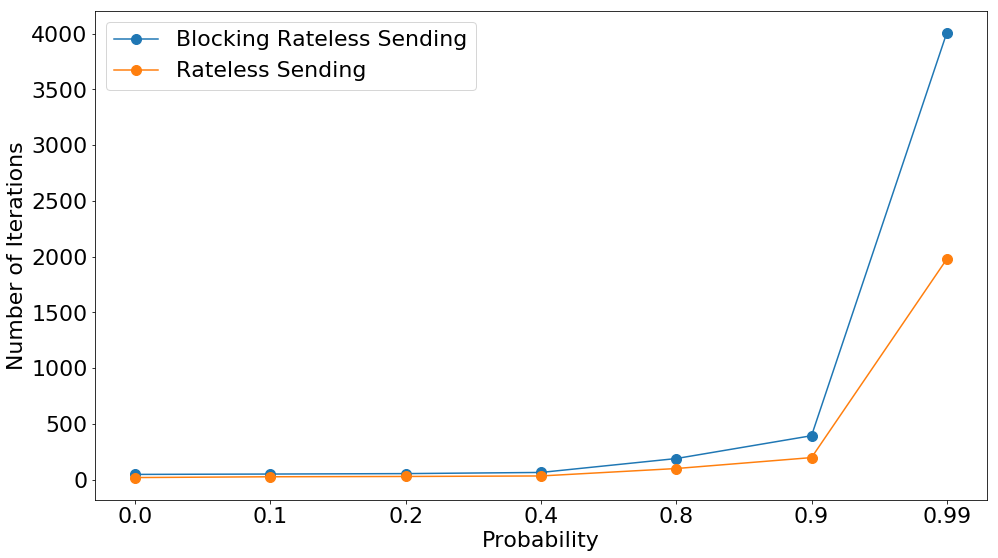
\includegraphics[width=8cm]{figures/big_font/block_comp.png}
\caption{Comparison of the blocking and non-blocking Rateless senders}
\label{graph:blockingvsnot}
\end{figure}

\begin{figure}[tp]
\centering
\noindent
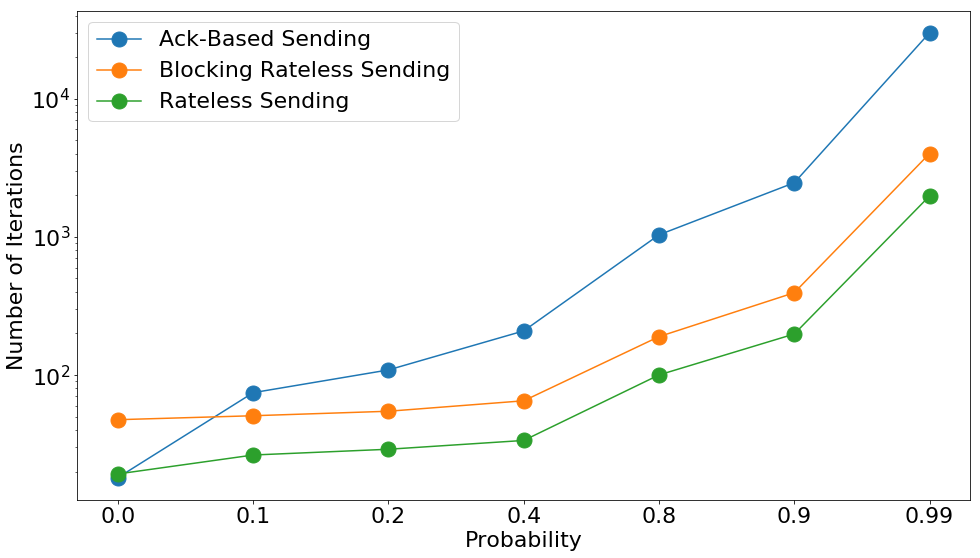
\includegraphics[width=8cm]{figures/big_font/triple_comp.png}
\caption{Comparison of the ACKing and two Rateless senders on a log y-axis}
\label{graph:ackvsratelessLOG}
\end{figure}

\section{Conclusion}
\textbf{LETS WRITE A REAL CONCLUSION}


One actionable avenue that is not explored in this paper is a way of merging our ideas presented here with the existing internet infrastructure. This path, while most likely less clean and more complex could provide a path to  increasing the robustness of the national broadcast system.


\textbf{Acknowledgements:} We thank Murphy McCauley for helping us get started with this idea. We also are grateful for Nick Weaver, who helped us solidify our security model.


% \begin{figure}[tp]
% \centering
% \includegraphics{figures/mouse}
% \caption{\blindtext}
% \end{figure}
% And we need some citation here\cite{floyd1993random, stoica2001chord}